% !TeX root = ../main.tex

\section{Introduzione}

\begin{frame}{Motivazione}
    \textbf{Problema}:
    \begin{itemize}
        \item Esecuzione manuale dei task del processo di sviluppo
        \item Errore umano
        \item Scarsa collaborazione/comunicazione
        \item Complessità di gestione e configurazione degli strumenti di sviluppo
        \item Ripetizione codice tra diverse piattaforme
        \item Ripetizione task tra diverse piattaforme
        \item Tempi lunghi di rilascio
        \item ...
    \end{itemize}
    
    \vspace{5mm}
    
    \textbf{Soluzione}:
    \begin{itemize}
        \item DevOps
        \item Applicazioni Multipiattaforma
    \end{itemize}
        
    \vspace{5mm}
    
    \textbf{Obiettivo}: Dimostrare l'efficacia della cultura DevOps e del paradigma multipiattaforma, adottati per lo sviluppo di applicazioni mobile
\end{frame}

\begin{frame}{DevOps}
    \begin{columns}[onlytextwidth]
        \begin{column}{0.45\textwidth}
            \textbf{Principi}:
            \begin{itemize}
                \item Comunicazione/Collaborazione
                \item Automazione
                \item Monitoraggio
            \end{itemize}
            \vspace{3mm}
            \textbf{Vantaggi}:
            \begin{itemize}
                \item Risparmio di tempo e risorse
                \item Tempi di consegna minori
                \item Maggiore qualità
            \end{itemize}
            \vspace{3mm}
            \textbf{Tecniche}:
            \begin{itemize}
                \item Continuous Integration
                \item Continuous Delivery
                \item Continuous Inspection
                \item ...
            \end{itemize}
        \end{column}
        \begin{column}{0.55\textwidth}
             \begin{figure}[H]
                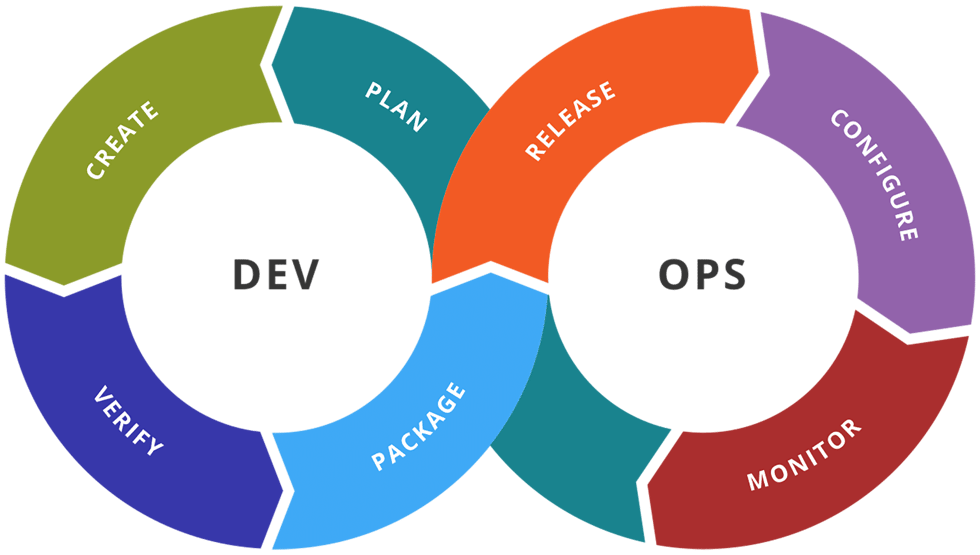
\includegraphics[width=1\textwidth]{img/Devops-toolchain.png}
            \end{figure}
        \end{column}
    \end{columns}
\end{frame}

\begin{frame}{Applicazioni Multipiattaforma}
    
\end{frame}